\documentclass[aspectratio=169,10pt]{beamer}

% metroplis theme
\usetheme[numbering=counter,progressbar=none]{metropolis}

\usefonttheme{default} 
\usepackage[sfdefault]{FiraSans}
\usepackage{FiraMono}

\usepackage{tikz}
\usetikzlibrary{arrows.meta,positioning,calc,fit}
\usepackage{amsmath}
\usepackage{booktabs}
\usepackage{xcolor}
\usepackage{pgfpages}

\usepackage[many]{tcolorbox} 

\setbeameroption{hide notes}

% Color Palette
\definecolor{mDarkTeal}{HTML}{03383b}  % Header bg, Title text, Blue box border
\definecolor{mLightGray}{HTML}{FAFAFA} % Main slide background
\definecolor{tealBorder}{HTML}{6A9A9D} % Teal box border
\definecolor{tealBg}{HTML}{F2F6F6}     % Teal box body background
\definecolor{blueBg}{HTML}{EBECEE}     % Blue box body background
\definecolor{mText}{HTML}{041f25}      % Default text color
\definecolor{mRed}{HTML}{f97171}       

\setbeamercolor{normal text}{fg=mText,bg=mLightGray}
\setbeamercolor{frametitle}{fg=white,bg=mDarkTeal}
\setbeamercolor{title separator}{fg=mDarkTeal}
\setbeamercolor{itemize item}{fg=mDarkTeal}
\setbeamercolor{itemize subitem}{fg=mDarkTeal}
\setbeamercolor{alerted text}{fg=mRed}

\setbeamertemplate{itemize item}{\textbullet}
\setbeamertemplate{itemize subitem}{$\circ$}

\setbeamerfont{frametitle}{size=\large,series=\normalfont} 
\setbeamerfont{title}{size=\LARGE,series=\normalfont}
\setbeamerfont{subtitle}{size=\large,series=\normalfont}
\setbeamerfont{author}{size=\normalsize}

% ---------- Custom Info Boxes (matching screenshots exactly) ----------
\newtcolorbox{tealbox}[1]{
  colback=tealBg,
  colframe=tealBorder,
  coltitle=white,
  title={#1},
  arc=3pt,
  boxrule=1.5pt,
  left=6pt, right=6pt, top=4pt, bottom=4pt,
  fonttitle=\normalsize,
  fontupper=\footnotesize,
  boxsep=2pt
}

\newtcolorbox{bluebox}[1]{
  colback=blueBg,
  colframe=mDarkTeal,
  coltitle=white,
  title={#1},
  arc=3pt,
  boxrule=1.5pt,
  left=6pt, right=6pt, top=4pt, bottom=4pt,
  fonttitle=\normalsize,
  fontupper=\footnotesize,
  boxsep=2pt
}

% TikZ styles
\tikzset{
  arr/.style={-{Latex[length=2.2mm]}, thick, mDarkTeal!75},
  bigarr/.style={-{Latex[length=3mm]}, very thick, mDarkTeal!80},
  gpu/.style={font=\footnotesize\bfseries, text=mDarkTeal},
  shard/.style={draw=#1!80!black, fill=#1!13, rounded corners=2pt, thick,
    minimum width=0.80cm, minimum height=0.45cm, font=\scriptsize,
    text=#1!60!black, align=center},
  stage/.style={draw=#1!80!black, fill=#1!11, rounded corners=5pt, thick,
    minimum width=2.55cm, minimum height=0.72cm, align=center,
    font=\footnotesize, text=mDarkTeal},
  callout/.style={draw=mDarkTeal!18, fill=blueBg!80, rounded corners=5pt,
    text width=5.2cm, align=left, inner sep=6pt, font=\footnotesize},
  mini/.style={draw=mDarkTeal!18, fill=blueBg!75, rounded corners=4pt,
    text width=4.55cm, align=left, inner sep=5pt, font=\scriptsize},
  take/.style={draw=mDarkTeal!80!black, fill=tealBg, rounded corners=7pt, thick,
    text width=13.4cm, minimum height=0.54cm, align=center,
    inner sep=3.5pt, font=\small, text=mDarkTeal}
}
\newcommand{\takeaway}[1]{\begin{center}\begin{tikzpicture}\node[take]{#1};\end{tikzpicture}\end{center}}

% ---------- Title Page Info ----------
\title{Full Sharded Data Parallel}
\subtitle{Lorem Ipsum}
\author{Utshav Saha\\[0.5cm]\footnotesize sahaushno@gmal.com}
\date{} % Empty date to match the reference image

\begin{document}

% ================================================================
% Title Frame
\begin{frame}[plain] % 'plain' removes header/footer for the title page
  \maketitle
\end{frame}

% ================================================================
\begin{frame}[t]{11. Sharding: split one big thing into pieces}
\transfade[duration=0.2]
\begin{columns}[T,onlytextwidth]
\column{0.50\textwidth}
\vspace{0.15cm}
\begin{tikzpicture}[x=1cm,y=1cm]
  \node[font=\normalsize\bfseries] at (0,2.8) {One large model state};
  \draw[rounded corners=9pt, draw=mDarkTeal, fill=tealBg, very thick] (-2.0,1.75) rectangle (2.0,2.35);
  \node[font=\large\bfseries,text=mDarkTeal] at (0,2.05) {MODEL STATE};
  \only<2->{
    \draw[bigarr] (0,1.55) -- (0,0.92);
    \node[font=\normalsize\bfseries] at (0,0.65) {Break it into shards};
    \foreach \x/\c/\s in {-1.5/mDarkTeal/$S_0$,-0.5/tealBorder/$S_1$,0.5/orange/$S_2$,1.5/violet/$S_3$}{
      \node[shard=\c, minimum width=0.84cm,minimum height=0.52cm] at (\x,-0.15) {\s};
    }
  }
  \only<3->{
    \foreach \x/\g in {-1.5/GPU 0,-0.5/GPU 1,0.5/GPU 2,1.5/GPU 3}{
      \draw[arr] (\x,-0.48) -- (\x,-0.90);
      \node[gpu,font=\scriptsize\bfseries] at (\x,-1.18) {\g};
    }
  }
\end{tikzpicture}

\column{0.47\textwidth}
\vspace{0.2cm}
\begin{bluebox}{Story intuition}
In games, shards are small pieces that together complete one item. FSDP uses the same idea for training state.
\end{bluebox}
\vspace{0.12cm}
\begin{itemize}
  \item<2-> Split one large state into pieces.
  \item<3-> Give different pieces to different GPUs.
  \item<4-> Reconstruct a full piece of the model only when computation needs it.
\end{itemize}
\end{columns}
\vspace{0.08cm}
\only<4->{\takeaway{FSDP starts by \textbf{splitting} model state instead of \textbf{replicating} it.}}
\end{frame}

% ================================================================
\begin{frame}[t]{12. What exactly is sharded?}
\transfade[duration=0.2]
\begin{columns}[T,onlytextwidth]
\column{0.48\textwidth}
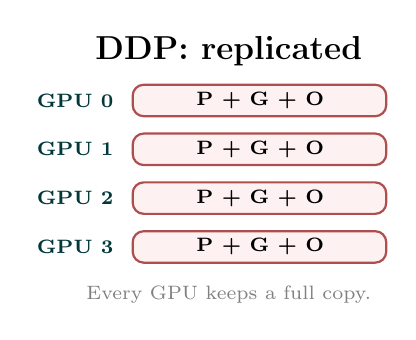
\begin{tikzpicture}[x=1cm,y=1cm]
  \node[font=\bfseries\large] at (0,2.8) {DDP: replicated};
  \foreach \i/\y in {0/2.18,1/1.56,2/0.94,3/0.32}{
    \node[gpu,font=\scriptsize\bfseries] at (-1.95,\y) {GPU \i};
    \draw[rounded corners=4pt,draw=mRed!70!black,fill=mRed!10,thick] (-1.22,\y-0.20) rectangle (2.00,\y+0.20);
    \node[font=\scriptsize\bfseries] at (0.40,\y) {P + G + O};
  }
  \node[font=\scriptsize,text=gray,align=center] at (0,-0.28) {Every GPU keeps a full copy.};
\end{tikzpicture}

\column{0.48\textwidth}
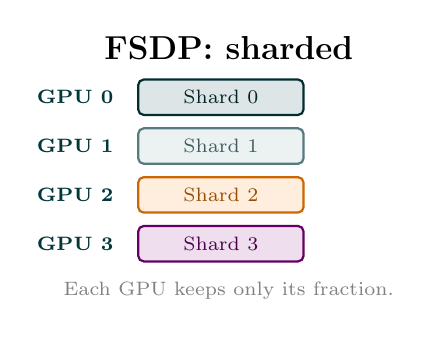
\begin{tikzpicture}[x=1cm,y=1cm]
  \node[font=\bfseries\large] at (0,2.8) {FSDP: sharded};
  \only<2->{
  \foreach \i/\y/\c/\s in {0/2.18/mDarkTeal/Shard 0,1/1.56/tealBorder/Shard 1,2/0.94/orange/Shard 2,3/0.32/violet/Shard 3}{
    \node[gpu,font=\scriptsize\bfseries] at (-1.95,\y) {GPU \i};
    \node[shard=\c, minimum width=2.1cm] at (-0.10,\y) {\s};
  }
  \node[font=\scriptsize,text=gray,align=center] at (0,-0.28) {Each GPU keeps only its fraction.};
  }
\end{tikzpicture}
\end{columns}
\vspace{0.08cm}
\only<3->{
\begin{center}
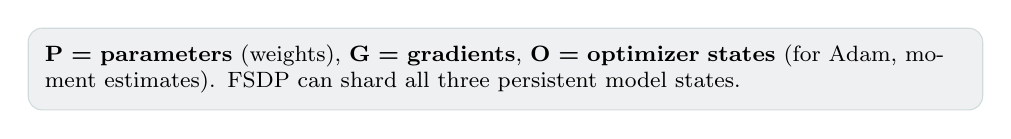
\begin{tikzpicture}
  \node[callout,text width=11.7cm] {\textbf{P = parameters} (weights), \textbf{G = gradients}, \textbf{O = optimizer states} (for Adam, moment estimates). FSDP can shard all three persistent model states.};
\end{tikzpicture}
\end{center}}
\vspace{-0.06cm}
\only<4->{\takeaway{Idealized persistent model-state memory per GPU scales roughly as $\frac{P+G+O}{N}$.}}
\end{frame}

% ================================================================
\begin{frame}[t]{13. The first problem: a layer cannot compute from one shard}
\transfade[duration=0.2]
\begin{columns}[T,onlytextwidth]
\column{0.50\textwidth}
\vspace{0.18cm}
\begin{tikzpicture}[x=1cm,y=1cm]
  \node[gpu] at (-1.25,2.35) {GPU 0 owns only};
  \node[shard=mDarkTeal,minimum width=1.1cm,minimum height=0.60cm] (w0) at (0.60,2.35) {$W_0$};
  \node[font=\scriptsize,text=gray] at (0,1.82) {one piece of a layer's weight tensor};
  \only<2->{
    \node[draw=mRed!80!black,fill=mRed!10,rounded corners=7pt,very thick,minimum width=3.5cm,minimum height=0.95cm,align=center] (calc) at (0,0.78) {Layer operation\\[-1mm] $y=Wx$};
    \draw[bigarr] (w0) -- (calc);
    \node[font=\Huge\bfseries,text=mRed] at (2.35,0.78) {?};
  }
  \only<3->{\node[font=\footnotesize,align=center] at (0,-0.15) {$W$ means the \textbf{complete} tensor,\\not only $W_0$.};}
\end{tikzpicture}

\column{0.47\textwidth}
\vspace{0.25cm}
\only<2->{\begin{tealbox}{The tension}
Sharding saves memory, but the current layer normally needs its full parameter tensor to run the matrix operations.
\end{tealbox}}
\vspace{0.15cm}
\only<3->{
\begin{center}
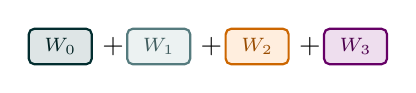
\begin{tikzpicture}
  \node[shard=mDarkTeal] at (0,0) {$W_0$};
  \node at (0.67,0) {$+$};
  \node[shard=tealBorder] at (1.25,0) {$W_1$};
  \node at (1.92,0) {$+$};
  \node[shard=orange] at (2.50,0) {$W_2$};
  \node at (3.17,0) {$+$};
  \node[shard=violet] at (3.75,0) {$W_3$};
\end{tikzpicture}
\end{center}}
\end{columns}
\vspace{0.08cm}
\only<4->{\takeaway{So FSDP must \textbf{temporarily collect} the missing parameter shards before computation.}}
\end{frame}

% ================================================================
\begin{frame}[t]{14. All-Gather: temporarily rebuild the current FSDP unit}
\transfade[duration=0.2]
\begin{center}
\begin{tikzpicture}[x=1cm,y=1cm]
  \node[font=\normalsize\bfseries] at (0,2.75) {Before: each GPU owns one shard};
  \foreach \x/\gpu/\c/\s in {-4.6/GPU 0/mDarkTeal/$W_0$,-1.55/GPU 1/tealBorder/$W_1$,1.55/GPU 2/orange/$W_2$,4.6/GPU 3/violet/$W_3$}{
    \node[gpu] at (\x,2.18) {\gpu};
    \node[shard=\c,minimum width=0.9cm,minimum height=0.52cm] at (\x,1.62) {\s};
  }
  \only<2->{
    \node[stage=orange,minimum width=3.15cm] (ag) at (0,0.72) {ALL-GATHER};
    \foreach \x in {-4.6,-1.55,1.55,4.6}{\draw[arr] (\x,1.30) -- (ag.north);}
  }
  \only<3->{
    \node[font=\normalsize\bfseries] at (0,-0.05) {After: full parameter for the current unit is available on every GPU};
    \foreach \x/\gpu in {-4.6/GPU 0,-1.55/GPU 1,1.55/GPU 2,4.6/GPU 3}{
      \node[gpu,font=\scriptsize\bfseries] at (\x,-0.65) {\gpu};
      \foreach \dx/\c in {-0.42/mDarkTeal,-0.14/tealBorder,0.14/orange,0.42/violet}{
        \draw[rounded corners=1pt,draw=\c!80!black,fill=\c!14,thick] (\x+\dx-0.12,-1.28) rectangle (\x+\dx+0.12,-0.92);
      }
      \node[font=\scriptsize,text=gray] at (\x,-1.55) {$W_0W_1W_2W_3$};
    }
  }
\end{tikzpicture}
\end{center}
\vspace{0.03cm}
\only<4->{\takeaway{All-Gather: \textbf{shards $\rightarrow$ full parameters}, but only for the unit currently being computed.}}
\end{frame}

% ================================================================
\begin{frame}[t]{15. Forward pass: gather, compute, reshard}
\transfade[duration=0.2]
\vspace{0.25cm}
\begin{center}
\begin{tikzpicture}[node distance=0.95cm]
  \node[stage=mDarkTeal] (s) {Sharded\\parameters};
  \only<2->{\node[stage=orange,right=of s] (ag) {All-Gather}; \draw[bigarr] (s) -- (ag);}
  \only<3->{\node[stage=tealBorder,right=of ag] (fw) {Forward\\compute}; \draw[bigarr] (ag) -- (fw);}
  \only<4->{\node[stage=violet,right=of fw] (rs) {Reshard}; \draw[bigarr] (fw) -- (rs);}

  \node[font=\scriptsize,text=gray] at ([yshift=-0.45cm]s.south) {low persistent memory};
  \only<3->{\node[font=\scriptsize,text=gray,align=center] at ([yshift=-0.52cm]fw.south) {full params exist\\briefly};}
  \only<4->{\node[font=\scriptsize,text=gray,align=center] at ([yshift=-0.52cm]rs.south) {discard non-owned\\pieces};}
\end{tikzpicture}
\end{center}
\vspace{0.35cm}
\only<5->{
\begin{columns}[T,onlytextwidth]
\column{0.48\textwidth}
\begin{bluebox}{Resharding}
After the forward computation, each GPU frees the full parameter and keeps only the shard it owns.
\end{bluebox}
\column{0.48\textwidth}
\begin{tealbox}{Why it saves memory}
The expensive full representation is temporary; the sharded representation is the persistent one.
\end{tealbox}
\end{columns}}
\vspace{0.05cm}
\only<6->{\takeaway{Forward = \textbf{All-Gather $\rightarrow$ compute $\rightarrow$ reshard}.}}
\end{frame}

% ================================================================
\begin{frame}[t,shrink=4]{16. Why gathering does not destroy the memory benefit}
\transfade[duration=0.2]
\begin{columns}[T,onlytextwidth]
\column{0.48\textwidth}
\vspace{0.12cm}
\begin{tikzpicture}[x=1cm,y=1cm]
  \node[font=\bfseries\large] at (0,2.85) {Layer-wise FSDP units};
  \foreach \i/\y in {1/2.20,2/1.57,3/0.94,4/0.31}{
    \draw[rounded corners=5pt,draw=gray!30,fill=blueBg!90] (-1.55,\y-0.21) rectangle (1.55,\y+0.21);
    \node[font=\footnotesize\bfseries] at (0,\y) {Transformer block \i};
  }
  \only<2>{\draw[rounded corners=5pt,draw=tealBorder,fill=tealBg,very thick] (-1.55,1.99) rectangle (1.55,2.41); \node[font=\footnotesize\bfseries,text=tealBorder!80!black] at (0,2.20) {Block 1: full};}
  \only<3>{\draw[rounded corners=5pt,draw=tealBorder,fill=tealBg,very thick] (-1.55,1.36) rectangle (1.55,1.78); \node[font=\footnotesize\bfseries,text=tealBorder!80!black] at (0,1.57) {Block 2: full};}
  \only<4->{\draw[rounded corners=5pt,draw=tealBorder,fill=tealBg,very thick] (-1.55,0.73) rectangle (1.55,1.15); \node[font=\footnotesize\bfseries,text=tealBorder!80!black] at (0,0.94) {Block 3: full};}
  \node[font=\scriptsize,text=gray,align=center] at (0,-0.28) {Other blocks can stay sharded.};
\end{tikzpicture}

\column{0.49\textwidth}
\vspace{0.2cm}
\only<2->{\begin{bluebox}{Important distinction}
FSDP gathers only the \textbf{current FSDP unit} (for example, one Transformer block), not the entire model.
\end{bluebox}}
\vspace{0.03cm}
\only<3->{\begin{center}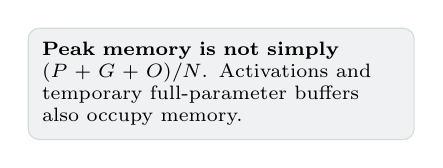
\begin{tikzpicture}\node[mini] {\textbf{Peak memory is not simply} $(P+G+O)/N$. Activations and temporary full-parameter buffers also occupy memory.};\end{tikzpicture}\end{center}}
\vspace{0.02cm}
\only<4->{\begin{center}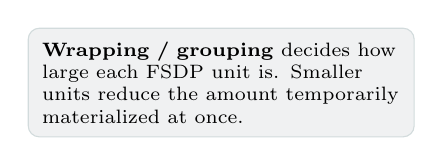
\begin{tikzpicture}\node[mini] {\textbf{Wrapping / grouping} decides how large each FSDP unit is. Smaller units reduce the amount temporarily materialized at once.};\end{tikzpicture}\end{center}}
\end{columns}
\vspace{-0.03cm}
\only<5->{\takeaway{FSDP controls peak memory by gathering \textbf{one unit at a time}.}}
\end{frame}

% ================================================================
\begin{frame}[t]{17. Backward pass: parameters are needed again}
\transfade[duration=0.2]
\begin{columns}[T,onlytextwidth]
\column{0.48\textwidth}
\vspace{0.10cm}
\begin{tikzpicture}[node distance=0.52cm]
  \node[stage=mDarkTeal,minimum width=3.25cm] (s) {Sharded parameters};
  \only<2->{\node[stage=orange,below=of s,minimum width=3.25cm] (ag) {All-Gather again}; \draw[bigarr] (s) -- (ag);}
  \only<3->{\node[stage=tealBorder,below=of ag,minimum width=3.25cm] (bw) {Backward compute}; \draw[bigarr] (ag) -- (bw);}
  \only<4->{\node[stage=mRed,below=of bw,minimum width=3.25cm] (grad) {Gradient contributions}; \draw[bigarr] (bw) -- (grad);}
\end{tikzpicture}

\column{0.49\textwidth}
\vspace{0.22cm}
\only<3->{\begin{tealbox}{Why gather again?}
Backpropagation needs the current layer's parameters to compute gradients with respect to inputs and weights.
\end{tealbox}}
\vspace{0.12cm}
\only<4->{\begin{bluebox}{New problem}
Each GPU processed different mini-batch data, so their gradient contributions must be synchronized before the optimizer update.
\end{bluebox}}
\end{columns}
\vspace{0.05cm}
\only<5->{\takeaway{Backward creates distributed gradient contributions; FSDP must combine them efficiently.}}
\end{frame}

% ================================================================
\begin{frame}[t]{18. Reduce-Scatter: combine gradients, then split again}
\transfade[duration=0.2]
\begin{columns}[T,onlytextwidth]
\column{0.49\textwidth}
\vspace{0.08cm}
\begin{tikzpicture}[x=1cm,y=1cm]
  \node[font=\normalsize\bfseries] at (0,2.7) {1. Gradient contributions};
  \foreach \x/\gpu/\c in {-1.8/GPU 0/mDarkTeal,-0.6/GPU 1/tealBorder,0.6/GPU 2/orange,1.8/GPU 3/violet}{
    \node[gpu,font=\scriptsize\bfseries] at (\x,2.08) {\gpu};
    \node[shard=\c] at (\x,1.60) {$g$};
  }
  \only<2->{\node[stage=tealBorder,minimum width=3.4cm] (reduce) at (0,0.65) {REDUCE: combine};
    \foreach \x in {-1.8,-0.6,0.6,1.8}{\draw[arr] (\x,1.30) -- (reduce.north);}}
  \only<3->{\node[stage=violet,minimum width=3.4cm] (scatter) at (0,-0.45) {SCATTER: redistribute}; \draw[arr] (reduce) -- (scatter);}
\end{tikzpicture}

\column{0.48\textwidth}
\vspace{0.08cm}
\only<3->{
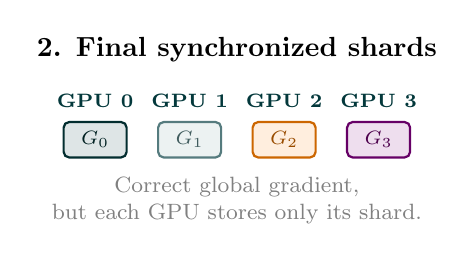
\begin{tikzpicture}[x=1cm,y=1cm]
  \node[font=\normalsize\bfseries] at (0,2.7) {2. Final synchronized shards};
  \foreach \x/\gpu/\c/\s in {-1.8/GPU 0/mDarkTeal/$G_0$,-0.6/GPU 1/tealBorder/$G_1$,0.6/GPU 2/orange/$G_2$,1.8/GPU 3/violet/$G_3$}{
    \node[gpu,font=\scriptsize\bfseries] at (\x,2.05) {\gpu};
    \node[shard=\c] at (\x,1.55) {\s};
  }
  \node[font=\footnotesize,text=gray,align=center] at (0,0.78) {Correct global gradient,\\but each GPU stores only its shard.};
\end{tikzpicture}}
\only<4->{\begin{tealbox}{Compare with DDP}
DDP typically uses \textbf{All-Reduce}: every rank ends with the full synchronized gradient. FSDP uses \textbf{Reduce-Scatter}: each rank ends with only its shard.
\end{tealbox}}
\end{columns}
\vspace{0.02cm}
\only<5->{\takeaway{Reduce-Scatter = \textbf{combine} gradient contributions, then \textbf{redistribute} only the owned shard.}}
\end{frame}

% ================================================================
\begin{frame}[t]{19. The complete FSDP training cycle}
\transfade[duration=0.2]
\begin{center}
\begin{tikzpicture}[x=1cm,y=1cm]
  % left-to-right top row
  \node[stage=mDarkTeal,minimum width=2.2cm] (p) at (-5.1,1.60) {Sharded\\params};
  \only<2->{\node[stage=orange,minimum width=2.2cm] (ag1) at (-2.55,1.60) {All-Gather}; \draw[bigarr] (p) -- (ag1);}
  \only<3->{\node[stage=tealBorder,minimum width=2.2cm] (fw) at (0,1.60) {Forward}; \draw[bigarr] (ag1) -- (fw);}
  \only<4->{\node[stage=violet,minimum width=2.2cm] (re) at (2.55,1.60) {Reshard}; \draw[bigarr] (fw) -- (re);}
  \only<5->{\node[stage=orange,minimum width=2.2cm] (ag2) at (5.1,1.60) {All-Gather}; \draw[bigarr] (re) -- (ag2);}

  % bottom row reversed
  \only<6->{\node[stage=tealBorder,minimum width=2.2cm] (bw) at (5.1,-0.10) {Backward}; \draw[bigarr] (ag2) -- (bw);}
  \only<7->{\node[stage=violet,minimum width=2.2cm] (rs) at (2.55,-0.10) {Reduce-Scatter}; \draw[bigarr] (bw) -- (rs);}
  \only<8->{\node[stage=mDarkTeal,minimum width=2.2cm] (g) at (0,-0.10) {Sharded\\grads}; \draw[bigarr] (rs) -- (g);}
  \only<9->{\node[stage=tealBorder,minimum width=2.2cm] (opt) at (-2.55,-0.10) {Optimizer\\update}; \draw[bigarr] (g) -- (opt);}
  \only<9->{\draw[bigarr] (opt) -- (-5.1,-0.10) -- (p.south); \node[font=\scriptsize,text=gray,align=center] at (-4.45,-0.10) {updated\\owned shard};}

  \only<10->{\node[callout,text width=10.6cm] at (0,-1.35) {At the optimizer step, each GPU already owns the matching \textbf{parameter shard + gradient shard + optimizer-state shard}, so it can update that shard locally.};}
\end{tikzpicture}
\end{center}
\vspace{-0.02cm}
\only<11->{\takeaway{Keep model state divided for memory; gather parameters briefly only when computation needs them.}}
\end{frame}

% ================================================================
\begin{frame}[t,shrink=2]{20. Final trade-off: memory down, communication up}
\transfade[duration=0.2]
\begin{columns}[T,onlytextwidth]
\column{0.51\textwidth}
\vspace{0.05cm}
\begin{tabular}{@{}lll@{}}
\toprule
 & \textbf{DDP} & \textbf{FSDP} \\
\midrule
Model state & Replicated & Sharded \\
Memory/GPU & Higher & Lower \\
Parameters & Already local & All-Gather \\
Gradient sync & All-Reduce & Reduce-Scatter \\
Main pressure & Memory & Communication \\
\bottomrule
\end{tabular}
\vspace{0.22cm}
\only<2->{\begin{bluebox}{The trade}
FSDP spends more network communication to reduce persistent GPU memory and make larger models trainable.
\end{bluebox}}

\column{0.46\textwidth}
\vspace{0.05cm}
\only<3->{
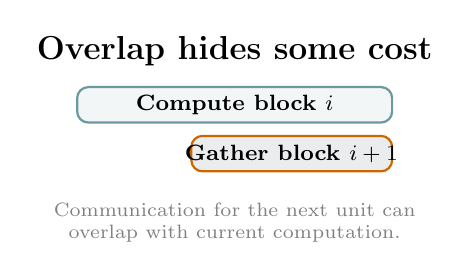
\begin{tikzpicture}[x=1cm,y=1cm]
  \node[font=\bfseries\large] at (0,2.45) {Overlap hides some cost};
  \draw[rounded corners=4pt,fill=tealBg,draw=tealBorder,thick] (-2.0,1.55) rectangle (2.0,2.00);
  \node[font=\footnotesize\bfseries] at (0,1.775) {Compute block $i$};
  \draw[rounded corners=4pt,fill=blueBg,draw=orange!80!black,thick] (-0.55,0.93) rectangle (2.0,1.38);
  \node[font=\footnotesize\bfseries] at (0.72,1.155) {Gather block $i+1$};
  \node[font=\scriptsize,text=gray,align=center] at (0,0.28) {Communication for the next unit can\\overlap with current computation.};
\end{tikzpicture}}
\only<4->{\begin{tealbox}{One-sentence summary}
\textbf{Shard most of the time; gather only when needed.}
\end{tealbox}}
\end{columns}
\vspace{0.02cm}
\only<5->{\takeaway{FSDP enables larger-model training by trading \textbf{memory} for \textbf{communication}.}}
\end{frame}

\end{document}